CloudMan will be used to manage an IaaS based computer center layout, as shown in figure~\ref{iaas}. The use cases naturally derive from this model. In this picture, each application comes with a backend which uses information from CloudMan to configure itself, respecting the allocations of resources to each defined user community.
\begin{figure}
\begin{center}
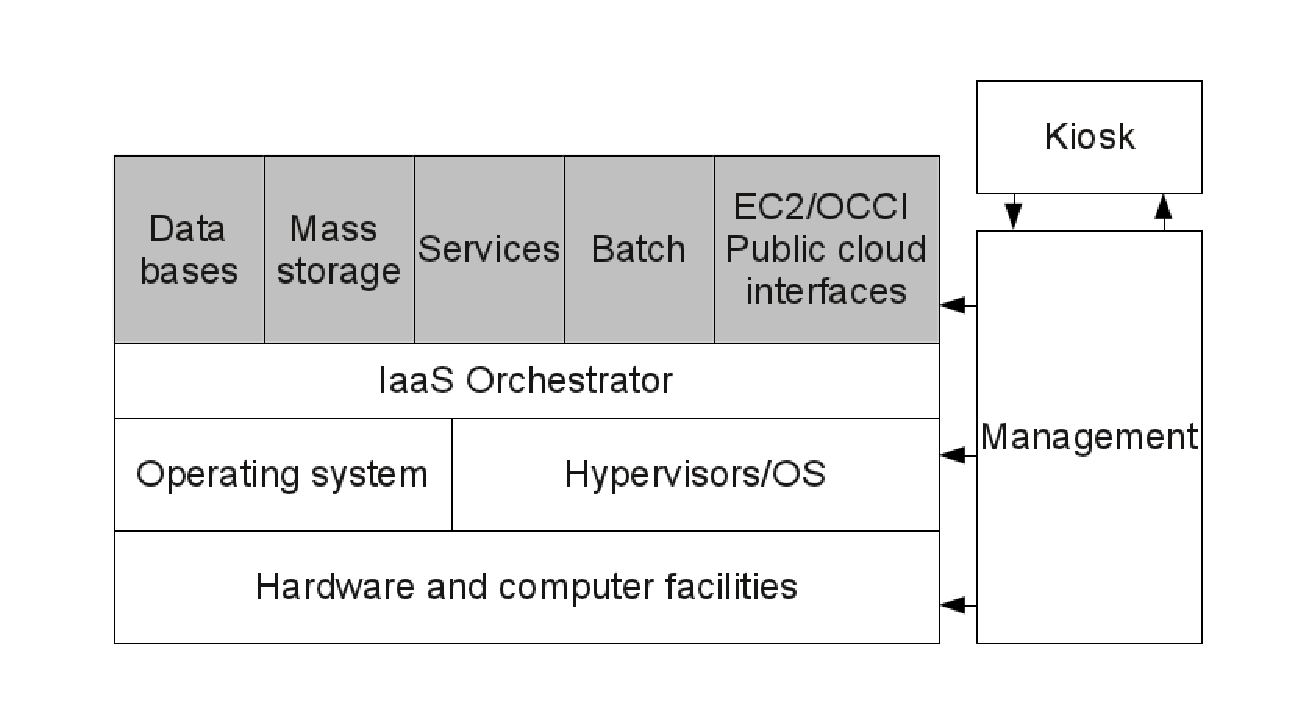
\includegraphics[width=\textwidth]{iaas.eps}
\caption{\label{iaas}Vision of a high level structure for an IaaS based computer center. CloudMan will be an essential part of the management layer for this model.}
\end{center}
\end{figure}
CloudMan must be capable to cope with the configuration of the use cases:
\begin{itemize}
\item Global allocations for individual IT services like 
\begin{itemize}
\item lxbatch resources, physical and virtual~\footnote{These correspond to different resource pools} 
\item public cloud resources for general use
\item storage resource pools for CASTOR and SWIFT
\item storage resource pools for virtual batch scratch and AFS cache space
\item physical resource pools for databases
\end{itemize}
\item The configuration of quotas per VO for an EC2 based self-service
\item The enforcement of quotas for reliable resources, based on total resources per VO by the resource manager
\item The configuration of shares for the batch farm VO project admins and subproject admins
\begin{itemize}
 \item The total resource allocation, typically in kSi2K for shared batch resources is done directly by the resource manager 
 \item The resource manager only defines a global allocation for each VO for resource pools used by the batch farm
 \item The difference between allocations done for the VOs and totally available resources for lxbatch are used for a public share
 \item The VO responsibles for projects and subprojects decide for which applications these resources are used. The fraction of resources allocated to batch processing is translated by the corresponding backend into a fair share value.
\end{itemize}
\end{itemize}

The following specific use cases are identified:
\begin{itemize}
\item new CPU resource have arrived for use by the self service
\item the fraction of SLC5 and SLC6 resources in lxbatch needs to be changed 

\end{itemize}

